\documentclass[a4paper,11pt]{article}
\usepackage[utf8]{inputenc}
\usepackage[T1]{fontenc}
\usepackage{lmodern}
\usepackage[frenchb]{babel}
\usepackage{graphicx}
\usepackage{color}
\usepackage{hyperref}
\usepackage{eurosym}
\usepackage{upgreek}
\usepackage{mathrsfs}
\usepackage{amssymb}
\usepackage{amsmath}
\usepackage{graphicx}
\usepackage{amsthm}
\usepackage{pgf,tikz}
\usetikzlibrary{arrows}
\usepackage{enumerate}
\usepackage{amsmath, amssymb, amsthm}
\usepackage{url}
\usepackage{multicol}
\newcommand{\eps}{\varepsilon}


\numberwithin{section}{part}
\renewcommand{\thesection}{\arabic{section}}

\setlength{\textwidth}{15cm} \setlength{\hoffset}{-1.50cm}
\setlength{\textheight}{630pt} \setlength{\voffset}{-1.4cm}

\selectlanguage{french}

\begin{document}

%% Debut couverture
 \setcounter{page}{0}
 \thispagestyle{empty}
\begin{center}
\sffamily
 {\LARGE \sc Semaine d'Etude Maths--Entreprises 4} \\
%\vspace*{0.5cm}
\vfill
 {\large  15--19 octobre 2012, Institut Henri Poincaré (Paris)}
\end{center}
\vfill
\begin{center}
 \LARGE \textsf{Observation de débris spatiaux}
\end{center}
\vspace*{0.5cm}
\begin{center}
 \large \sffamily
\begin{tabular}{cc}
         Nicolas \textsc{Bonnotte$^{a}$} & Maxime \textsc{Chupin$^{b}$} \\
         Tony \textsc{Février$^{c}$} & Antoine \textsc{Levitt$^{d}$} \\ 
         Benjamin \textsc{Marteau$^{e}$} & Vladimir \textsc{Salnikov$^{f}$}
   \end{tabular}
\end{center}
\vfill
\centerline{\footnotesize\it $^{a}$ Université Paris-Sud,\url{nicolas.bonnotte@math.u-psud.fr}}
\centerline{\footnotesize\it $^{b}$ Laboratoire de Mathématiques xxxxxxxxxxxxx, France}
\centerline{\footnotesize\it $^{c}$ Laboratoire de Mathématiques xxxxxxxxxxxxx, France}
\centerline{\footnotesize\it $^{d}$ Université Paris Dauphine, \url{levitt@ceremade.dauphine.fr}}
\centerline{\footnotesize\it $^{e}$ Laboratoire de Mathématiques
  xxxxxxxxxxxxx, France}
\centerline{\footnotesize\it $^{f}$ Laboratoire de Mathématiques xxxxxxxxxxxxx, France}

% \begin{multicols}{2}
% \participant{Nicolas Bonnotte}{doctorant à l'Université Paris-Sud}{nicolas.bonnotte@math.u-psud.fr}
% \participant{Maxime Chupin}{}{}
% \participant{Tony Février}{}{}
% \participant{Antoine Levitt}{doctorant à l'Université Paris Dauphine}{levitt@ceremade.dauphine.fr}
% \participant{Benjamin Marteau}{}{}
% \participant{Vladimir Salnikov}{}{}
% % rajoutez vos affiliations :
% % \participant{Prénom nom}{Affiliation}{Adresse électronique}
% \end{multicols}

\vfill

\hspace{1cm}Sujet propos\'e par~:
\begin{center}
\begin{tabular}{cc}

\includegraphics[scale=.4]{LOGO_EADS_ASTRIUM.jpg} 
\end{tabular}
\end{center}
\begin{center}
  \large \sffamily Correspondant : Max \textsc{Lecerf} (EADS)
\end{center}
\vfill
\vspace{3cm}
\begin{center}
\begin{tabular}{ccc}

\includegraphics[scale=0.9]{logo_GDR_ME}&

\includegraphics[scale=1.0]{logo_CNRS}&

\includegraphics[scale=0.05]{logo_AMIES}

\includegraphics[scale=0.4]{logo_LMV}
\end{tabular}
\end{center}
%% Fin couverture

\newpage
 \setcounter{page}{0}
\thispagestyle{empty}
\begin{center}

\abstract{blabla......}
\vfill
Mots clés :

\vfill
Num\'ero de publication : SEME00X-201X-0X-X
\end{center}
\newpage


\section{Contexte}

Ce travail a été réalisé dans le cadre de la 4\ieme{} 
Semaine d'étude mathématiques et entreprises (\textsc{seme}), qui s'est tenue à
dans les locaux de l'Institut Henri Poincaré (\textsc{ihp}) à Paris du lundi 15
au vendredi 19 octobre 2012. Le groupe souhaite remercier les
organisateurs de la \textsc{seme}, ainsi que Astrium et plus précisément Max
Cerf pour avoir proposé ce sujet, que nous avons trouvé intéressant et
riche.

% \begin{multicols}{2}
% \participant{Nicolas Bonnotte}{doctorant à l'Université Paris-Sud}{nicolas.bonnotte@math.u-psud.fr}
% \participant{Maxime Chupin}{}{}
% \participant{Tony Février}{}{}
% \participant{Antoine Levitt}{doctorant à l'Université Paris Dauphine}{levitt@ceremade.dauphine.fr}
% \participant{Benjamin Marteau}{}{}
% \participant{Vladimir Salnikov}{}{}
% % rajoutez vos affiliations :
% % \participant{Prénom nom}{Affiliation}{Adresse électronique}
% \end{multicols}



\section{Introduction}



%\section{Observation du débris}

\renewcommand{\phi}{\varphi}

\newcommand{\TD}{T_\text{d}}
\newcommand{\omegaD}{\omega_\text{d}}
\newcommand{\iD}{i_\text{d}}
\newcommand{\altitudeD}{r}
\newcommand{\rayonD}{\rayonT+\altitudeD}

\newcommand{\TT}{T_\text{t}}
\newcommand{\omegaT}{\omega_\text{t}}
\newcommand{\iT}{i_\text{t}}
\newcommand{\rayonT}{R}

\newcommand{\referentiel}{\mathcal{R}}

\section{Observabilité d'une orbite}

\subsection{Référentiel et notations}

Supposons qu'au temps $t=0$, on puisse voir au centre du télescope une certaine orbite, et donc potentiellement les débris qui s'y trouveraient. Pendant combien de temps pourra-t-on encore la voir ? Et, quand elle aura disparue, pendant combien de temps l'aura-t-on vue au total ?

On se place dans un référentiel $\referentiel = (O,\vec{e}_x,\vec{e}_y,\vec{e}_z)$ dont le centre est le centre de la Terre, tel que $(O,\vec{e}_x,\vec{e}_y)$ soit le plan de l'équateur. Notons $\iT \in [-\frac{\pi}{2}, \frac{\pi}{2}]$ l'inclinaison du télescope vis-à-vis de l'équateur, et $\phi \in [0,\pi]$ sa latitude : $\iT = \frac{\pi}{2} - \phi$, et $\phi=0$ correspond au pôle Nord, $\phi = \pi$ au pôle Sud. En notant  $\rayonT$ le rayon de la Terre et $\omegaT = \frac{2\pi}{\TT}$ la pulsation du télescope, les coordonnées de ce dernier dans notre référentiel $\referentiel$  sont :
\[ 
\overrightarrow{OT} = \rayonT \vec{u} \qquad \text{avec} \qquad \vec{u}(t) = \left(\begin{array}{c}
\cos(\omegaT t) \cos(\iT) \\
\sin(\omegaT t) \cos(\iT) \\
\sin(\iT)
\end{array}
\right).
\]
Supposons que l'orbite soit un cercle de centre $O$, de rayon $\rayonD$, dans un plan incliné d'un angle $\iD \in [0, \frac{\pi}{2}]$ vis-à-vis de l'équateur et de direction normale
\[ 
\vec{n} =  \left(\begin{array}{c}
 \sin(\iD)\cos(\theta) \\
\sin(\iD)\sin(\theta) \\
 \cos(\iD) 
\end{array}
\right).
\]
%L'orbite se trouve donc dans le plan $(O, \vec{u}, \vec{v})$, avec
%\[ 
%\vec{u} =  \left(\begin{array}{c}
% -\sin(\theta) \\
%\cos(\theta) \\
%0 
%\end{array}
%\right)
%\qquad \text{et} \qquad
%\vec{v} = \vec{n} \wedge \vec{u} =  \left(\begin{array}{c}
% -\cos(\iD) \cos(\theta) \\
% -\cos(\iD)\sin(\theta) \\
%  \sin(\iD)
%\end{array}
%\right)
%\]
À $t=0$, le télescope coupe le plan de l'orbite, et cela entraîne $\vec{n}\cdot \vec{u} = 0$. L'angle $\theta$ doit donc vérifier la relation
\[ \cos(\theta) = - \frac{\sin(\iT)\cos(\iD)}{\cos(\iT)\sin(\iD)}.\]

On note $\alpha$ le demi-angle de d'ouverture du télescope, ou plutôt le demi-angle qui serait celui sous lequel un observateur placé au centre de la Terre verrait la même chose à l'altitude $\altitudeD$ que le télescope. Si $\alpha_0$ est l'ouverture réelle du télescope, on a (voir \autoref{nicolas:alpha}) :
\[ \alpha = \frac{\rayonT}{\rayonD} \alpha_0 \approx 0,1\text{\degres}.\]

\begin{figure}
\begin{center}
\scriptsize
\def\figurewidth{0.6\linewidth}
\newlength{\unit}
\newlength{\width}
\setlength{\width}{\figurewidth}
\setlength{\unit}{0.0926\width}
%\setlength{\unit}{1cm}
%\setlength{\unit}{\texwidth}

\definecolor{xdxdff}{rgb}{0.49,0.49,1}
\definecolor{qqwuqq}{rgb}{0,0.39,0}
\definecolor{qqqqcc}{rgb}{0,0,0.8}
\definecolor{qqqqff}{rgb}{0,0,1}
\begin{tikzpicture}[line cap=round,line join=round,>=triangle 45,x=\unit,y=\unit]
\clip(4.11,-0.63) rectangle (10.8,5.62);
\draw [shift={(5,3)},color=qqwuqq,fill=qqwuqq,fill opacity=0.1] (0,0) -- (49.79:0.75) arc (49.79:90:0.75) -- cycle;
\draw [shift={(5,0)},color=qqwuqq,fill=qqwuqq,fill opacity=0.1] (0,0) -- (72.58:0.75) arc (72.58:90:0.75) -- cycle;
\draw [color=red, densely dotted] (5,0) circle (5\unit);
\draw [color=red] (5,5) arc (90:72:5\unit);
\draw [color=qqqqcc] (5,0) circle (3\unit);
\draw[dashed] (5,3)-- (5,0);
\draw (5,5)-- (5,3);
\draw[dashed] (5,0)-- (6.5,4.77);
\draw (5,3)-- (6.5,4.77);
\draw (4.5,4.12) node[anchor=north west] {$r$};
\draw (4.45,1.84) node[anchor=north west] {$R$};
\begin{scriptsize}
\fill [color=black] (5,0) circle (1.5pt);
\fill [color=red] (5,5) circle (1pt);
\fill [color=black] (5,3) circle (1.5pt);
\draw[color=qqqqff] (4.75,3.25) node {$T$};
\fill [color=red] (6.5,4.77) circle (1pt);
\draw[color=qqwuqq] (5.625,3.25) node {$\alpha_0$};
\draw[color=qqwuqq] (5.375,0.25) node {$\alpha$};
\fill [color=black] (5.75,4.94) circle (1.5pt);
\draw[color=red] (6.07,5.15) node {$D$};
\end{scriptsize}
\end{tikzpicture}

\caption{Rapport entre les angles $\alpha$ et $\alpha_0$} \label{nicolas:alpha}
\end{center}
\end{figure}


\subsection{Calcul approché de la durée journalière d'observation}

Supposons que l'orbite apparaisse dans la visée du télescope avec un angle $\psi$ vis-à-vis de l'horizontale. Elle balaye la fenêtre d'observation avec une vitesse $\omegaT \sin(\psi)$ (voir \autoref{nicolas:fenetre}). Il lui faut donc un temps $\tau_0$ pour traverser entièrement celle-ci, avec $\tau_0$ donné par la formule
\[ \tau_0 = \frac{2\alpha}{\omegaT \sin(\psi)}.\]
Cet angle $\psi$ est l'angle entre le vecteur vitesse du télescope $T$ et celui d'un débris $D$ situé sur l'orbite. 
%On connait déjà $\overrightarrow{OT}$ ; quant à $\overrightarrow{OD}$, on sait qu'il se déplace dans un plan $(O, \vec{f}_1, \vec{f}_2)$ perpendiculaire à $\vec{n}$ sur un cercle de rayon $\rayonD$ de centre $O$ et de vitesse angulaire $\omegaD = \frac{2\pi}{\TD}$, et que $O$, $T$ et $D$ sont alignés pour $t=0$. Ceci nous suffit pour obtenir :
%\[ \overrightarrow{OD} = (\rayonD)\vec{v} \qquad \text{avec} \qquad \vec{v} = \cos(\omegaD t) \vec{f}_1 + \sin(\omegaD t) \vec{f}_2\]
%si du moins
%\[ 
%\vec{f}_1 =  \left(
%	\begin{array}{c}
%		\cos(\iT) \\
%		0\\
%		\sin(\iT)
%	\end{array}
%\right) \quad \text{et} \quad \vec{f}_2 =  \frac{1}{\cos(\iT)} \left(
%	\begin{array}{c}
%		\sin(\iT) \sqrt{\sin(\iD)^2 - \sin(\iT)^2} \\
%		\cos(\iD) \\
%		-\cos(\iT) \sqrt{\sin(\iD)^2 - \sin(\iT)^2}
%	\end{array}
%\right).
%\]
%Par conséquent, l'angle $\psi$ est donné par la formule
On peut montrer que
\[ 
\cos(\psi) = \frac{\cos(\iD)}{\cos(\iT)}.
\]
Puisqu'il y a deux observations par jour, la durée journalière d'observation de l'orbite est
\[ \tau = 2\tau_0 = \frac{4\alpha\cos(\iT)}{\sqrt{\sin(\iD)^2 - \sin(\iT)^2}}.\]
Malheureusement, cette formule n'a probablement pas de sens si $\iD$ et $\iT$ sont trop rapprochés, ou si $\iT$ est trop proche de $\frac{\pi}{2}$. C'est pourquoi nous allons maintenant essayer une autre méthode, exacte celle-ci.

\begin{figure}
\begin{center}
\scriptsize
\def\figurewidth{0.6\linewidth}
%\newlength{\unit}
%\newlength{\width}
\setlength{\width}{\figurewidth}
\setlength{\unit}{0.3\width}



\definecolor{qqzzqq}{rgb}{0,0.6,0}
\definecolor{ffqqqq}{rgb}{1,0,0}
\definecolor{qqqqcc}{rgb}{0,0,0.8}
\definecolor{uququq}{rgb}{0.25,0.25,0.25}

\begin{tikzpicture}[line cap=round,line join=round,>=triangle 45,x=\unit,y=\unit]
\draw[color=black, dashed] (-1,0) -- (1,0);
%\foreach \x in {-1,-0.5,0.5,1}
%\draw[shift={(\x,0)},color=black] (0pt,2pt) -- (0pt,-2pt) node[below] {\footnotesize $\x$};
%\draw[color=black] (0,-1.36) -- (0,1.28);
%\foreach \y in {-1,-0.5,0.5,1}
%\draw[shift={(0,\y)},color=black] (2pt,0pt) -- (-2pt,0pt) node[left] {\footnotesize $\y$};
%\draw[color=black] (0,0.125) node[right] {\footnotesize $O$};
\clip(-1.44,-1.36) rectangle (1.31,1.28);
\draw [shift={(-1.25,-1)},color=qqqqcc,fill=qqqqcc,fill opacity=0.1] (0,0) -- (0:0.18) arc (0:75.07:0.18) -- cycle;
\draw [->] (-1.25,-1) -- (-0.85,-1);
\draw [->] (-1.25,-1) -- (-1.05,-0.25);
\draw [color=red,domain=-.486:0.0133] plot(\x,{(--0.19--0.75*\x)/0.2});
\draw [color=red,densely dotted,domain=-0.0368:-.5295] plot(\x,{(--0.19--0.75*(\x+0.05))/0.2});
\draw [color=red,dotted,domain=-0.0876:-.5720] plot(\x,{(--0.19--0.75*(\x+0.1))/0.2});
\draw [color=red,loosely dotted,domain=-.13926:-.6138] plot(\x,{(--0.19--0.75*(\x+0.15))/0.2});
%\draw [color=qqzzqq,domain=-1.44:1.31] plot(\x,{(-0-0.2*\x)/0.75});
\draw [->, color=red] (-0.43,-0.67) -- (-0.06,-0.77);
%\draw [->] (-0.43,-0.67) -- (-0.2,0.18);
\begin{scriptsize}
\fill [color=black] (0,0) circle (1.5pt);
%\draw[color=uququq] (0.05,0.08) node {$O$};
\draw[color=black] (-0.87,-0.92) node {$\omegaT$};
\draw[color=black] (-1,-0.61) node {$\omegaD$};
\draw[color=qqqqcc] (-1.15,-0.92) node {$\psi$};
\draw[color=black] (0.13,-0.66) node {$\omegaT \sin(\psi)$};
%\draw[color=black] (0.15,-0.3) node {$\omegaD + \omegaT \cos(\psi)$};
\draw [line width=1pt] (0,0) circle (1);
\end{scriptsize}
\end{tikzpicture}
\caption{Fenêtre d'observation} \label{nicolas:fenetre}
\end{center}
\end{figure}



\subsection{Calcul exact de la durée journalière d'observation}

On rappelle que $\alpha$ désigne le demi-angle d'observation en équivalent pour un observateur situé au centre de la Terre. L'orbite est donc visible si et seulement si
\[ -\sin(\alpha) \leq \vec{n} \cdot \vec{u} \leq \sin(\alpha).\]
Notons $t_\pm$ les deux instants les plus proches de $t=0$ tels que
\[  \vec{n} \cdot \vec{u}(t_+) = \sin(\alpha) \qquad \text{et} \qquad  \vec{n} \cdot \vec{u}(t_-) = -\sin(\alpha).\] 
Puisque $\alpha$ est petit, on a donc :
\begin{multline*}
\cos(\omegaT t_\pm) \cos(\iT) \sin(\iD) \cos(\theta) + \sin(\omegaT t_\pm) \cos(\iT)\sin(\iD)\sin(\theta)
 = \pm\alpha -  \sin(\iT)\cos(\iD).
\end{multline*}
Ceci entraîne
\[ \cos(\theta - \omegaT t_\pm) = \cos(\theta) \pm  \frac{\alpha}{\cos(\iT)\sin(\iD)}.\]
Puisque $t_\pm$ est petit, 
\[ \sin(\theta) \omegaT t_\pm - \frac{1}{2} \cos(\theta) \left(\omegaT t_\pm\right)^2 = \pm  \frac{\alpha}{\cos(\iT)\sin(\iD)},\]
et on obtient donc
\[ \omegaT t_\pm = A - \sqrt{A^2 \mp \frac{\alpha\cos(\iT)\sin(\iD)}{\sin^2(\iT)\cos^2(\iD)}} \qquad \text{avec} \qquad A=\frac{\cos(\iT)\sin(\iD)\sqrt{\sin^2(\iD)-\sin^2(\iT)}}{\sin^2(\iT)\cos^2(\iD)}\]
Le taux d'observation sur une journée est  $ \tau = 2(t_+ - t_-)$, en convenant que $t_\pm = 0$ lorsque la formule donnant $t_\pm$ n'a pas de sens. On a :
\[ \tau = \frac{2}{\omegaT} \left(  \sqrt{A^2 + \frac{\alpha\cos(\iT)\sin(\iD)}{\sin^2(\iT)\cos^2(\iD)}} - \sqrt{A^2 - \frac{\alpha\cos(\iT)\sin(\iD)}{\sin^2(\iT)\cos^2(\iD)}} \right).\]
En particulier,
\begin{align*}
  \tau =  &\frac{2}{\omegaT}\sqrt{\frac{\alpha}{\cos(\iD)\sin(\iD)}} & \text{si $\iD = \iT$}, \\
  \tau =  &\frac{2}{\omegaT}\frac{\alpha}{\sqrt{\sin(\iD)^2 - \sin(\iT)^2}} & \text{si $\iD > \iT \gg \alpha$}.
\end{align*}%

\begin{figure}
\scriptsize
\begin{center}
\def\svgwidth{0.5\linewidth}
 \input{figures/observabilite3.pdf_tex}
 \vspace*{-2em}
\caption{Durée journalière d'observation (en minutes)} \label{nicolas:observabilite}
\end{center}
\end{figure}%

La \autoref{nicolas:observabilite} montre le nombre de minutes par jour où l'orbite est visible. Cette durée ne dépend que de $\iT$ et de $\iD$. Lorsque $\iD=\iT=0$ ou $\iD=\iT=\frac{\pi}{2}$, l'orbite est en permanence visible : le premier cas correspond au télescope situé sur l'équateur avec une orbite équatoriale, le second au télescope au pôle Nord avec une orbite polaire. Lorsque $\iD < \iT$, l'orbite n'est pas assez inclinée et n'est donc jamais visible par le télescope, situé lui à une latitude trop élevée. Lorsque $\iD = \frac{\pi}{2}$ et $\iT = \frac{\pi}{4}$, c'est-à-dire pour une orbite polaire et un télescope à la latitude de Bordeaux, l'orbite est visible 96 secondes par jour. Lorsque $\iD = \frac{\pi}{2}$ et $\iT = 0$, c'est-à-dire pour une orbite polaire et un télescope à l'équateur, l'orbite n'est plus visible que 48 secondes par jour. 


\subsection{Partie de l'orbite observée chaque jour}

Lorsque l'on voit l'orbite durant un temps $\mathrm{d}t$, celle-ci tournant avec une vitesse $\omegaD$, on observe en fait une proportion $\mathrm{d}p = \frac{\omegaD}{2\pi} \mathrm{d} t = \frac{\mathrm{d}t}{\TD}$. La proportion de l'orbite observée par jour est donc
\[ p = \frac{\omegaD \tau}{2\pi} = \frac{\tau}{\TD}.\]
Si $\TD = 2 \text{h}$, pour une orbite polaire et un télescope à l'équateur on observe $p \approx 1 \%$ de l'orbite par jour. En supposant donc que l'on n'observe jamais deux fois les mêmes débris, et que ceux-ci sont répartis uniformément  sur l'orbite, on peut donc espérer observer $1 \%$ des débris par jours.






\section{Conditions d'éclairement}

Dans cette partie on se place dans un rep\`ere g\'eocentrique qui tourne \`a la vitesse de rotation de la Terre autour du soleil. Ainsi on peut voir le mouvement du soleil relativement \`a la Terre comme une simple variation de l'incidence $i_S$ de ces rayons.  La figure \ref{ombre} repr\'esente ce rep\`ere : la Terre est en rouge, la sph\`ere transparente est celle contenant le d\'ebris et en bleu, on observe le c\^one d'ombre g\'en\'er\'e par les rayons incidents. 

 \begin{figure}[h]\label{ombre}
    \centering
    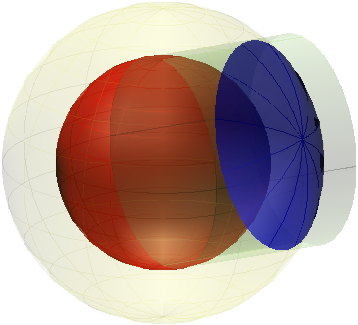
\includegraphics[width=.6\textwidth]{figures/ombre.pdf}
    \caption{Proportion de zone observable pendant un an}
 \end{figure}
 
\vspace{0.5cm} Ainsi les saisons sont déterminées par une variation de l'angle d'incidence entre le plan équatorial et les rayons solaires.
On modélise dans notre repère cette variation par $i_{S}(t)= i_{max}\cos(\omega_{s}t)$ où $i_{max}=23.75^o$ et $\displaystyle{\omega_s=\frac{2\pi}{T_s}}$. \\
 
L'objectif de cette partie est de d\'eterminer la proportion de ciel observable en prenant en compte les contraintes suivantes : 

\begin{itemize}
\item Le d\'ebris doit \^etre \'eclair\'e par le soleil. 
\item Le t\'elescope doit \^etre dans la nuit.
\end{itemize}

\vspace{0.5cm}

Ces deux contraintes s"int\'egrent au mod\'ele par l'interm\'ediaire de deux angles d\'ependant du temps $t$ : $\beta(t)$ repr\'esentant le c\^one d'ombre auquel ne doit pas appartenir le d\'ebris, $\delta(t)$ permettant de d\'elimiter la nuit du jour . Afin de mieux voir o\`u interviennent ces deux angles, on s'int\'eresse \`a deux coupes horizontales repr\'esent\'ees en rouge dans la figure \ref{coupehor}:
\begin{itemize}
\item celle incluant la trajectoire du t\'elescope (coupe de latitude $\varphi$).
\item celle contenant le cercle des points o\`u le d\'ebris sera observable par le t\'elescope (les intersections entre les droites du z\'enith du t\'elescope et la sph\`ere de motion du d\'ebris).
\end{itemize}

\begin{figure}\label{coupehor}
\begin{center}
\scriptsize
\def\figurewidth{0.6\linewidth}
% \documentclass[10pt]{article}
% \usepackage[utf8]{inputenc}
% \usepackage{pgf,tikz}
% \usetikzlibrary{arrows}
% \pagestyle{empty}
% \begin{document}
\definecolor{qqwuqq}{rgb}{0,0.39,0}
\definecolor{ffqqqq}{rgb}{1,0,0}
\definecolor{xdxdff}{rgb}{0.49,0.49,1}
\definecolor{qqqqff}{rgb}{0,0,1}
\definecolor{uququq}{rgb}{0.25,0.25,0.25}
\begin{tikzpicture}[line cap=round,line join=round,>=triangle 45,x=1.0cm,y=1.0cm]
\clip(-26.49,-38.19) rectangle (51.52,18.74);
\draw [shift={(0,0)},color=qqwuqq,fill=qqwuqq,fill opacity=0.1] (0,0) -- (0:3.39) arc (0:27.02:3.39) -- cycle;
\draw(0,0) circle (10cm);
\draw(0,0) circle (15.95cm);
\draw [domain=-26.49:51.52] plot(\x,{(--100-8.91*\x)/4.54});
\draw [domain=-26.49:51.52] plot(\x,{(-0--4.54*\x)/8.91});
\draw [color=ffqqqq,domain=-26.49:51.52] plot(\x,{(-7.24-0*\x)/-1});
\draw [color=ffqqqq,domain=-26.49:51.52] plot(\x,{(-4.54-0*\x)/-1});
\draw [domain=-26.49:51.52] plot(\x,{(-0-0*\x)/-10});
\draw (0,-38.19) -- (0,18.74);
\begin{scriptsize}
\fill [color=uququq] (0,0) circle (1.5pt);
\draw[color=uququq] (0.56,0.91) node {$A$};
\fill [color=qqqqff] (10,0) circle (1.5pt);
\draw[color=qqqqff] (10.45,0.91) node {$B$};
\fill [color=qqqqff] (14.21,7.24) circle (1.5pt);
\draw[color=qqqqff] (14.72,8.1) node {$D$};
\fill [color=xdxdff] (8.91,4.54) circle (1.5pt);
\draw[color=xdxdff] (9.43,5.45) node {$T$};
\draw[color=qqwuqq] (3.13,0.64) node {$\varphi$};
\end{scriptsize}
\end{tikzpicture}
% \end{document}

\caption{Rapport entre les angles $\alpha$ et $\alpha_0$} \label{alpha}
\end{center}
\end{figure}

Ces deux coupes horizontales sont celles des figures \ref{coupehorbeta} et \ref{coupehordelta}. Ainsi le t\'elescope doit non seulement \^etre hors du jour (il lui reste $\pi-2\delta(t)$ de p\'erim\`etre disponible) mais aussi il ne doit pas pointer dans le c\^one d'ombre (enlever $2\beta(t))$ de p\'erim\`etre.

\begin{figure}\label{coupehorbeta}
\begin{center}
\scriptsize
\def\figurewidth{0.6\linewidth}

\definecolor{qqwuqq}{rgb}{0,0.39,0}
\definecolor{uququq}{rgb}{0.25,0.25,0.25}
\definecolor{xdxdff}{rgb}{0.49,0.49,1}
\definecolor{qqqqff}{rgb}{0,0,1}
\begin{tikzpicture}[line cap=round,line join=round,>=triangle 45,x=1.0cm,y=1.0cm,scale=0.7]
\draw[->,color=black] (-5.76,0) -- (6.47,0);
\foreach \x in {-5,-4,-3,-2,-1,1,2,3,4,5,6}
\draw[shift={(\x,0)},color=black] (0pt,2pt) -- (0pt,-2pt) node[below] {\footnotesize $\x$};
\draw[->,color=black] (0,-4.44) -- (0,3.78);
\foreach \y in {-4,-3,-2,-1,1,2,3}
\draw[shift={(0,\y)},color=black] (2pt,0pt) -- (-2pt,0pt) node[left] {\footnotesize $\y$};
\draw[color=black] (0pt,-10pt) node[right] {\footnotesize $0$};
\clip(-5.76,-4.44) rectangle (6.47,3.78);
\draw [shift={(0,0)},color=qqwuqq,fill=qqwuqq,fill opacity=0.1] (0,0) -- (0:0.7) arc (0:22:0.7) -- cycle;
\draw(0,0) circle (3cm);
\draw(0,0) circle (2cm);
\draw [domain=-5.76:6.47] plot(\x,{(-0-0*\x)/2});
\draw (2.78,-4.44) -- (2.78,3.78);
\draw (0,0)-- (2.78,1.12);
\draw (0,0)-- (2.78,-1.12);
\begin{scriptsize}
\fill [color=qqqqff] (0,0) circle (1.5pt);
\draw[color=qqqqff] (-0.12,0.24) node {$O$};
\fill [color=xdxdff] (2,0) circle (1.5pt);
\draw[color=xdxdff] (2.1,0.16) node {$T$};
\fill [color=uququq] (0,2) circle (1.5pt);
\draw[color=uququq] (0.2,2.16) node {$N_1$};
\fill [color=uququq] (3,0) circle (1.5pt);
\draw[color=uququq] (3.1,0.16) node {$D$};
\fill [color=uququq] (0,-2) circle (1.5pt);
\draw[color=uququq] (0.09,-1.84) node {$S$};
\fill [color=xdxdff] (2.78,1.12) circle (1.5pt);
\draw[color=xdxdff] (2.88,1.28) node {$A$};
\fill [color=uququq] (2.78,-1.12) circle (1.5pt);
\draw[color=uququq] (2.87,-0.96) node {$B$};
\draw[color=qqwuqq] (0.56,0.11) node {$\beta$};
\end{scriptsize}
\end{tikzpicture}
\caption{Rapport entre les angles $\alpha$ et $\alpha_0$} \label{alpha}
\end{center}
\end{figure}

\begin{figure}\label{coupehordelta}
\begin{center}
\scriptsize
\def\figurewidth{0.6\linewidth}

\definecolor{qqwuqq}{rgb}{0,0.39,0}
\definecolor{uququq}{rgb}{0.25,0.25,0.25}
\definecolor{xdxdff}{rgb}{0.49,0.49,1}
\definecolor{qqqqff}{rgb}{0,0,1}
\begin{tikzpicture}[line cap=round,line join=round,>=triangle 45,x=1.cm,y=1.cm,scale=0.6]
\draw[->,color=black] (-5.76,0) -- (6.47,0);
\foreach \x in {-5,-4,-3,-2,-1,1,2,3,4,5,6}
\draw[shift={(\x,0)},color=black] (0pt,2pt) -- (0pt,-2pt) node[below] {\footnotesize $\x$};
\draw[->,color=black] (0,-4.44) -- (0,3.78);
\foreach \y in {-4,-3,-2,-1,1,2,3}
\draw[shift={(0,\y)},color=black] (2pt,0pt) -- (-2pt,0pt) node[left] {\footnotesize $\y$};
\draw[color=black] (0pt,-10pt) node[right] {\footnotesize $0$};
\clip(-5.76,-4.44) rectangle (6.47,3.78);
\draw [shift={(0,0)},color=qqwuqq,fill=qqwuqq,fill opacity=0.1] (0,0) -- (63.02:0.64) arc (63.02:90:0.64) -- cycle;
\draw(0,0) circle (3cm);
\draw (0,0)-- (1.36,2.67);
\draw (1.36,-4.44) -- (1.36,3.78);
\draw (0,0)-- (1.36,-2.67);
\begin{scriptsize}
\fill [color=qqqqff] (0,0) circle (1.5pt);
\draw[color=qqqqff] (-0.12,0.24) node {$O$};
\fill [color=xdxdff] (1.36,2.67) circle (1.5pt);
\draw[color=xdxdff] (1.47,2.84) node {$A$};
\fill [color=uququq] (1.36,-2.67) circle (1.5pt);
\draw[color=uququq] (1.46,-2.51) node {$B$};
\fill [color=uququq] (0,3) circle (1.5pt);
\draw[color=uququq] (0.11,3.17) node {$C$};
\draw[color=qqwuqq] (0.26,0.39) node {$\delta$};
\end{scriptsize}
\end{tikzpicture}
\caption{Rapport entre les angles $\alpha$ et $\alpha_0$} \label{alpha}
\end{center}
\end{figure}

La proportion de zone observable par le t\'elescope est donc donn\'ee par $$\displaystyle{p_{V}(t,\varphi)=\frac{\pi-2\beta(t)-2\delta(t)}{2\pi}}.$$ \\
\\
Des arguments de g\'eom\'etrie \'elementaires  nous permettent d'obtenir les formules suivantes pour ces deux angles caract\'eristiques : \\

\begin{itemize}
\item $\displaystyle{\beta(t)=\arccos\left(\frac{\sqrt{2rR+r^2}\cos(i_s(t))}{(R+r)\sin(\varphi)}\right)}$.
\item $\displaystyle{\delta(t)=\arcsin\left(\frac{|\tan(i_s(t))|}{\tan(\varphi)}\right)}$.
\end{itemize}

\vspace{0.5cm}
\noindent o\`u $R$ et $R+r$ d\'esignent respectivement le rayon de la Terre et de l'orbite du d\'ebris.\\

Munis de ces r\'esultats,  nous avons ainsi pu d\'eterminer pour chaque latitude $\varphi$ la moyenne de proportion de zone observable sur un an, le but \'etant de d\'eterminer la latitude id\'eale de placement du t\'elescope. \\

A SUIVRE AVEC LES FIGURES DEFINITIVES....


\section{Ergodicité}
Les calculs que nous avons faits donnent la probabilité $p$ qu'étant
donné un débris de paramètres $a_{D}$ et $i_{D}$ positionné
aléatoirement sur son orbite, il soit vu en un jour. La question qui
se pose maintenant est celle de l'indépendance des
observations. Peut-on considérer que l'observation au jour $J+1$ est
indépendante de l'observation au jour $J$ ? Si on regarde le ciel
pendant $N$ jours, le nombre de fois où le débris est vu suit-il une
loi binomiale $B(n,p)$, comme ce serait le cas si les observations
étaient indépendantes ? Si non, peut-on obtenir des estimations sur la
durée d'observation nécessaire pour voir le débris ?

La réponse mathématique à ces questions est délicate. Dans cette
partie, on introduit un modèle simplifié qui reprend néanmoins les
caractéristiques principales du problème réel, et on étudie le passage
à un modèle probabiliste. On considère un téléscope et un débris, et
on ignore les problèmes de visibilité dûs au soleil, ainsi que le
mouvement de précession.

Si la latitude du téléscope le permet, la zone d'observation du
téléscope croise l'orbite du débris deux fois par jour, tous les jours
aux mêmes heures $t_{1}$ et $t_{2}$. Pendant tout le temps où l'orbite
est visible, le débris parcourt un angle $\beta$ sur son orbite. Dans
le régime qui nous intéresse, $\beta \approx 10 \alpha$ : on
considérera donc l'approximation $\beta \gg \alpha$ où le téléscope
observe un point de l'orbite, et verra le débris si il traverse ce
point. Entre deux croisements de l'orbite et du téléscope, le débris
parcourt un angle $\theta$ sur son orbite. $\theta$ alterne entre deux
valeurs $\theta_{t_{1} \to t_{2}}$ et $\theta_{t_{2} \to t_{1}}$. Ces
deux valeurs ne varient pas de jour en jour (même si on prend en
compte la précession). On simplifie le modèle en considérant que
$\theta_{t_{1} \to t_{2}} = \theta_{t_{2} \to t_{1}} = \theta$, ou de
façon équivalente qu'on n'observe qu'une fois sur les deux
opportunités par jour. Cette simplification n'affecte pas les
caractéristiques principales du modèle.

% \begin{center}
%   \definecolor{qqwuqq}{rgb}{0,0.39,0}
\definecolor{ffqqqq}{rgb}{1,0,0}
\definecolor{qqqqff}{rgb}{0,0,1}
\begin{tikzpicture}[line cap=round,line join=round,>=triangle 45,x=1.0cm,y=1.0cm]
\clip(-2.46,-1.58) rectangle (5.82,5.82);
\draw [shift={(1,2)},color=qqwuqq,fill=qqwuqq,fill opacity=0.1] (0,0) -- (0:2) arc (0:74.05:2) -- cycle;
\draw [shift={(1,2)},color=qqwuqq,fill=qqwuqq,fill opacity=0.1] (0,0) -- (143.2:2) arc (143.2:161.57:2) -- cycle;
\draw [color=ffqqqq] (1,2) circle (3.16cm);
\draw (1,2)-- (-2,3);
\draw (1,2)-- (-1.53,3.89);
\draw (1,2)-- (4.16,2);
\draw (1,2)-- (1.87,5.04);
\begin{scriptsize}
\fill [color=qqqqff] (1,2) circle (1.5pt);
\fill [color=black] (4.16,2) circle (1.5pt);
\draw[color=black] (5.0,2.26) node {$\text{Débris à t}$};
\fill [color=black] (1.87,5.04) circle (1.5pt);
\draw[color=black] (3.54,5.3) node {$\text{Débris à }t+Tobs$};
\draw[color=qqwuqq] (2.22,2.6) node {$\theta$};
\draw[color=qqwuqq] (0.64,2.48) node {$\alpha$};
\end{scriptsize}
\end{tikzpicture}

%   \input{ergodic}
  
%   (refaire meilleure figure)
% \end{center}

On pose
\begin{align}
  \label{modelejouet}
  \theta_{n} = (\theta_{0} + n \theta) \mod 1,
\end{align}
où $\theta_{0}$ est une phase initiale aléatoirement distribuée, et
$\theta$ est un paramètre. On considère qu'on a observation du débris
au jour $n$ si $0 \in [\theta_{n}, \theta_{n}+\beta]$, où $\beta$ est
la fraction de l'orbite parcourue par le débris pendant une
journée. On appelle $N(n)$ le nombre cumulé d'observations du débris
au jour $n$. On sait que si $\theta$ est irrationnel, alors
\begin{align}
  \label{largenumbers}
  \lim_{n\to\infty} \frac{N(n)} n = \beta.
\end{align}
(théorème d'équirépartition\footnote{\url{http://en.wikipedia.org/wiki/Equidistribution_theorem}})

Ce théorème est un analogue de la loi des grand nombres : en temps
grand, la fréquence d'observation du débris est égale à la proportion
du cercle observée par le téléscope. Le problème est que ce théorème
ne nous apporte pas d'informations concrètes sur la vitesse de
convergence de cette limite, qui nous permettrait d'obtenir des
conclusions pratiques. 

Si au lieu du modèle déterministe \eqref{modelejouet} on utilise un
modèle probabiliste où $\theta_{n}$ est une variable aléatoire
distribuée uniformément entre 0 et 1, alors $N(n)$ suit la loi
binomiale $B(n,\beta)$. Cela implique par exemple
\begin{align}
  P(N(n) \geq 1) = 1 - (1-\beta)^{n}.
\end{align}

La question est de savoir si des estimations semblables peuvent être
obtenues pour le modèle déterministe. Ce problème est un sujet d'étude
en théorie ergodique. Un théorème de Kesten\cite{kesten} montre que si
$\theta$, $\theta_{0}$ sont distribués uniformément sur $[0,1]$ et
$\beta$ est irrationnel, alors le nombre $N(n)$ d'observations en $n$
itérations suit pour $n$ grand la loi
\begin{align}
  N(n) \approx n \beta + \frac {\rho_{0}}\beta \log n\; \mathcal C,
\end{align}
où $\rho_{0}$ est une constante universelle\footnote{le théorème est également
valable pour $\beta$ rationnel, mais alors le facteur correctif en
$\rho_{0}$ dépend non-trivialement de $\beta$}, et $\mathcal C$ est
la distribution de Cauchy, de densité
\begin{align}
  f_{\mathcal C}(x) = \frac 1 \pi \frac 1 {1+x^{2}}
\end{align}

La distribution de Cauchy a des queues extrêmement épaisses (sa
moyenne n'est même pas définie). En particulier, le théorème implique
que, pour $n$ grand,
\begin{align}
  P(N(n) = 0) \approx \frac {\log n}{\rho \beta \pi n}
\end{align}

Cette décroissance en $\frac {\log n} n$ est extrêmement lente (elle
est à comparer avec la décroissance exponentielle en $(1-p)^{n}$ si
les observations étaient indépendantes d'un jour à l'autre).

% Les simulations numériques que nous avons effectuées montrent que
% l'approximation aléatoire est une bonne approximation, mais ne permet
% pas de rendre compte de certains phénomènes (certains débris mettent
% plus de temps à se laisser observer que dans le modèle aléatoire). La
% question de la compréhension fine de ce phénomène est une question
% ouverte intéressante du point de vue à la fois théorique (théorie
% ergodique) et pratique (pour se prémunir de la possibilité de ne pas
% observer certains débris aussi rapidement que ce que prédit l'approche
% probabiliste).

\section{Résultats numériques}

\section{Conclusion}
Limitations, perspectives :
\begin{itemize}
\item Orbites circulaires (modèle adaptable)
\item $T_{\text{débris}} \ll T_{\text{terre}}$ : erreur de $10\%$ pour
  orbites basses (héliosynchrones), pas valable pour orbites hautes
  (géostationnaires)
\item Limites du modèle probabiliste, qui semble pourtant assez
  pertinent. Modèle effectif qui rendrait compte du synchronisme
  partiel des phénomènes ?
\item Pas de prise en compte fine du téléscope (quelle position
  choisir pour un bon $\alpha$ ?)
\item Simulations numériques naïves (timestep trop grand quand orbite
  en vue donc sous-estimation de la visibilité, et timestep trop petit
  quand orbite pas en vue donc temps de calcul beaucoup trop
  important). Essayer de prédire les intersections, et
  ``fast-forward'' de la simulation.
\end{itemize}



%\section*{Remerciements}



\begin{thebibliography}{99}
\bibitem{kesten}{Kesten, H. (1960). Uniform distribution mod 1. The Annals of
    Mathematics, 71(3), 445-471.}
\end{thebibliography}
\end{document}
